\documentclass[]{article}
\usepackage{lmodern}
\usepackage{amssymb,amsmath}
\usepackage{ifxetex,ifluatex}
\usepackage{fixltx2e} % provides \textsubscript
\ifnum 0\ifxetex 1\fi\ifluatex 1\fi=0 % if pdftex
  \usepackage[T1]{fontenc}
  \usepackage[utf8]{inputenc}
\else % if luatex or xelatex
  \ifxetex
    \usepackage{mathspec}
  \else
    \usepackage{fontspec}
  \fi
  \defaultfontfeatures{Ligatures=TeX,Scale=MatchLowercase}
\fi
% use upquote if available, for straight quotes in verbatim environments
\IfFileExists{upquote.sty}{\usepackage{upquote}}{}
% use microtype if available
\IfFileExists{microtype.sty}{%
\usepackage{microtype}
\UseMicrotypeSet[protrusion]{basicmath} % disable protrusion for tt fonts
}{}
\usepackage[margin=1in]{geometry}
\usepackage{hyperref}
\hypersetup{unicode=true,
            pdftitle={Module 1.1},
            pdfauthor={Getting started: working with objects},
            pdfborder={0 0 0},
            breaklinks=true}
\urlstyle{same}  % don't use monospace font for urls
\usepackage{color}
\usepackage{fancyvrb}
\newcommand{\VerbBar}{|}
\newcommand{\VERB}{\Verb[commandchars=\\\{\}]}
\DefineVerbatimEnvironment{Highlighting}{Verbatim}{commandchars=\\\{\}}
% Add ',fontsize=\small' for more characters per line
\usepackage{framed}
\definecolor{shadecolor}{RGB}{248,248,248}
\newenvironment{Shaded}{\begin{snugshade}}{\end{snugshade}}
\newcommand{\KeywordTok}[1]{\textcolor[rgb]{0.13,0.29,0.53}{\textbf{#1}}}
\newcommand{\DataTypeTok}[1]{\textcolor[rgb]{0.13,0.29,0.53}{#1}}
\newcommand{\DecValTok}[1]{\textcolor[rgb]{0.00,0.00,0.81}{#1}}
\newcommand{\BaseNTok}[1]{\textcolor[rgb]{0.00,0.00,0.81}{#1}}
\newcommand{\FloatTok}[1]{\textcolor[rgb]{0.00,0.00,0.81}{#1}}
\newcommand{\ConstantTok}[1]{\textcolor[rgb]{0.00,0.00,0.00}{#1}}
\newcommand{\CharTok}[1]{\textcolor[rgb]{0.31,0.60,0.02}{#1}}
\newcommand{\SpecialCharTok}[1]{\textcolor[rgb]{0.00,0.00,0.00}{#1}}
\newcommand{\StringTok}[1]{\textcolor[rgb]{0.31,0.60,0.02}{#1}}
\newcommand{\VerbatimStringTok}[1]{\textcolor[rgb]{0.31,0.60,0.02}{#1}}
\newcommand{\SpecialStringTok}[1]{\textcolor[rgb]{0.31,0.60,0.02}{#1}}
\newcommand{\ImportTok}[1]{#1}
\newcommand{\CommentTok}[1]{\textcolor[rgb]{0.56,0.35,0.01}{\textit{#1}}}
\newcommand{\DocumentationTok}[1]{\textcolor[rgb]{0.56,0.35,0.01}{\textbf{\textit{#1}}}}
\newcommand{\AnnotationTok}[1]{\textcolor[rgb]{0.56,0.35,0.01}{\textbf{\textit{#1}}}}
\newcommand{\CommentVarTok}[1]{\textcolor[rgb]{0.56,0.35,0.01}{\textbf{\textit{#1}}}}
\newcommand{\OtherTok}[1]{\textcolor[rgb]{0.56,0.35,0.01}{#1}}
\newcommand{\FunctionTok}[1]{\textcolor[rgb]{0.00,0.00,0.00}{#1}}
\newcommand{\VariableTok}[1]{\textcolor[rgb]{0.00,0.00,0.00}{#1}}
\newcommand{\ControlFlowTok}[1]{\textcolor[rgb]{0.13,0.29,0.53}{\textbf{#1}}}
\newcommand{\OperatorTok}[1]{\textcolor[rgb]{0.81,0.36,0.00}{\textbf{#1}}}
\newcommand{\BuiltInTok}[1]{#1}
\newcommand{\ExtensionTok}[1]{#1}
\newcommand{\PreprocessorTok}[1]{\textcolor[rgb]{0.56,0.35,0.01}{\textit{#1}}}
\newcommand{\AttributeTok}[1]{\textcolor[rgb]{0.77,0.63,0.00}{#1}}
\newcommand{\RegionMarkerTok}[1]{#1}
\newcommand{\InformationTok}[1]{\textcolor[rgb]{0.56,0.35,0.01}{\textbf{\textit{#1}}}}
\newcommand{\WarningTok}[1]{\textcolor[rgb]{0.56,0.35,0.01}{\textbf{\textit{#1}}}}
\newcommand{\AlertTok}[1]{\textcolor[rgb]{0.94,0.16,0.16}{#1}}
\newcommand{\ErrorTok}[1]{\textcolor[rgb]{0.64,0.00,0.00}{\textbf{#1}}}
\newcommand{\NormalTok}[1]{#1}
\usepackage{graphicx,grffile}
\makeatletter
\def\maxwidth{\ifdim\Gin@nat@width>\linewidth\linewidth\else\Gin@nat@width\fi}
\def\maxheight{\ifdim\Gin@nat@height>\textheight\textheight\else\Gin@nat@height\fi}
\makeatother
% Scale images if necessary, so that they will not overflow the page
% margins by default, and it is still possible to overwrite the defaults
% using explicit options in \includegraphics[width, height, ...]{}
\setkeys{Gin}{width=\maxwidth,height=\maxheight,keepaspectratio}
\IfFileExists{parskip.sty}{%
\usepackage{parskip}
}{% else
\setlength{\parindent}{0pt}
\setlength{\parskip}{6pt plus 2pt minus 1pt}
}
\setlength{\emergencystretch}{3em}  % prevent overfull lines
\providecommand{\tightlist}{%
  \setlength{\itemsep}{0pt}\setlength{\parskip}{0pt}}
\setcounter{secnumdepth}{0}
% Redefines (sub)paragraphs to behave more like sections
\ifx\paragraph\undefined\else
\let\oldparagraph\paragraph
\renewcommand{\paragraph}[1]{\oldparagraph{#1}\mbox{}}
\fi
\ifx\subparagraph\undefined\else
\let\oldsubparagraph\subparagraph
\renewcommand{\subparagraph}[1]{\oldsubparagraph{#1}\mbox{}}
\fi

%%% Use protect on footnotes to avoid problems with footnotes in titles
\let\rmarkdownfootnote\footnote%
\def\footnote{\protect\rmarkdownfootnote}

%%% Change title format to be more compact
\usepackage{titling}

% Create subtitle command for use in maketitle
\newcommand{\subtitle}[1]{
  \posttitle{
    \begin{center}\large#1\end{center}
    }
}

\setlength{\droptitle}{-2em}

  \title{Module 1.1}
    \pretitle{\vspace{\droptitle}\centering\huge}
  \posttitle{\par}
    \author{Getting started: working with objects}
    \preauthor{\centering\large\emph}
  \postauthor{\par}
      \predate{\centering\large\emph}
  \postdate{\par}
    \date{September 2018}


\begin{document}
\maketitle

NOTE: this module borrows heavily from an R short course developed by a
team at Colorado State University. - Thanks to Perry Williams for
allowing us to use these materials!!

Welcome to the 2018 R bootcamps! Let's get started!!

\subsection{Load script for module
\#1.1}\label{load-script-for-module-1.1}

\begin{enumerate}
\def\labelenumi{\arabic{enumi}.}
\item
  Click \href{module1_1.R}{here} to download the script! Save the script
  to a convenient folder on your laptop. I recommend making a new folder
  to store all your scripts from this bootcamp!
\item
  Load your script in RStudio. To do this, open RStudio and click on the
  folder icon in the toolbar at the top and load your script. Your
  RStudio interface should be divided into four quadrants. On the top
  left is your \textbf{script}, on the bottom left is your
  \textbf{console}, on the top right is your \textbf{Environment}, and
  on the bottom left are some helper interfaces that let you get help,
  load packages, view plots, etc. Basically, RStudio provides all the
  functionality you need to develop, debug and execute R code!
\end{enumerate}

Let's get started!!!

\begin{figure}
\centering
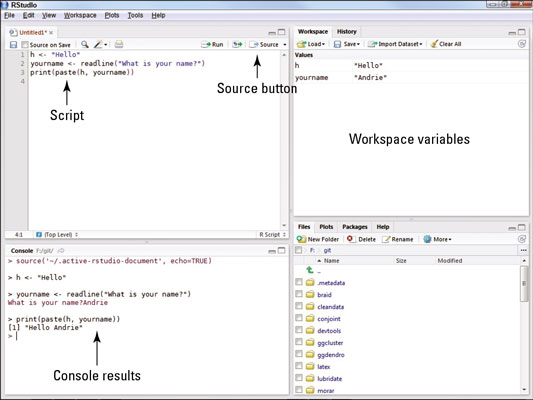
\includegraphics{rstudio1.jpg}
\caption{}
\end{figure}

\subsection{Explore the R console}\label{explore-the-r-console}

The R console (what you see if you opened R directly without going
through RStudio) is a \textbf{command line} interface. That means you
give R a command to run and R executes that command. This is the heart
of R- all the rest of RStudio consist of wrappers to help us make the
most effective use of the console! In fact, after this short demo you
will rarely interact directly with the console!

The R console is located in the left half or bottom left of the RStudio
interface (see figure above).

\begin{enumerate}
\def\labelenumi{\arabic{enumi}.}
\item
  Click on the console just to the right of one of the
  ``\textgreater{}'' prompts.
\item
  You can use the console like a calculator. For example, type
  \texttt{2+2} at the prompt and hit enter. What does R do?
\item
  Now hit the ``up'' arrow. The R console remembers all previous
  commands in this \textbf{session}, which allows you to re-run commands
  relatively easily. However, if you accidentally hit the ``up'' arrow
  you lose everything you had been typing!
\item
  Any command that is preceded by a pound sign (\#) is ignored by the R
  console. Try typing \texttt{\#\ 2+2} and hitting ``Enter''. Nothing
  happens, right?
\end{enumerate}

\subsubsection{Let's create our first
object}\label{lets-create-our-first-object}

Objects are assigned a value using R's \textbf{assignment operator},
which looks like a left arrow (\texttt{\textless{}-}). Type the
following statement into the console:

\begin{Shaded}
\begin{Highlighting}[]
\NormalTok{Batmans_butler <-}\StringTok{ 'Alfred Pennyworth'}
\end{Highlighting}
\end{Shaded}

Then hit ``Enter''. What does R return?

NOTHING!

BUT\ldots{}. check the \textbf{Environment}, or \textbf{Workspace}
window (top right of RStudio interface). You should see that you now
have a new \textbf{object} in your environment, called
``Batmans\_butler'', which stores a \textbf{text string}: ``Alfred
Pennyworth''.

Now type \texttt{print(Batmans\_butler)}\footnote{NOTE: \texttt{print()}
  is an \textbf{R function} that comes with base R. It takes the name of
  an object as its \textbf{argument} and it responds by printing the
  contents of that object. We'll get more into R functions shortly.}
into the R console and hit ``Enter''. What happens? \footnote{RStudio
  has a useful auto-type feature, which can save you lots of time and
  headaches. After you've typed the first couple letters (e.g.,
  ``bat''), RStudio will suggest ``Batmans\_butler'' and you can just
  hit ``Enter'' to complete the object name! The auto-type feature,
  unlike R, is not case sensitive!}

If you enter the name of an object at the command line, R automatically
prints the value of the object- you don't need to use the
\texttt{print()} function\ldots{} Try it: type \texttt{Batmans\_butler}
into the R console and hit ``Enter''. R dutifully returns the name of
Bruce Wayne's loyal and tireless butler, best friend and surrogate
father figure.

\subsection{Graduating to R Scripts}\label{graduating-to-r-scripts}

You will quickly realize that although the command-line R console is
nice for some things, there is a much better way to develop R code. That
is by storing a sequential set of commands as a text file. This text
file (the standard is to use the ``.R'' extension) is called an
\textbf{R script}. The top left quadrant of the RStudio interface is
dedicated to developing R scripts. The file you downloaded at the
beginning of this module is an R script.

The first few lines (commands) of the script are preceded by pound
signs. R doesn't do anything with these commands- they are called
\textbf{comments}, and they help to keep code clear, organized and
understandable to human readers. \emph{use comments early and often-
they are tremendously valuable}.

\begin{enumerate}
\def\labelenumi{\arabic{enumi}.}
\item
  Click on the top of the script (first line of comments). To
  \textbf{run} a line of code, press the ``Ctrl'' key (or the
  ``Command'' key) and hit ``Enter''. R will then run that line through
  the console. But of course, nothing happens because it's a comment and
  not meant to be interpreted by a machine\footnote{RStudio has several
    helpful keyboard shortcuts to make running lines of code easier.
    \href{https://support.rstudio.com/hc/en-us/articles/200711853-Keyboard-Shortcuts}{Check
    this website} for a comprehensive set of keyboard shortcuts}.
\item
  Click on a blank line in the script and type \texttt{2+2}. Now hit
  ``Ctrl+Enter'' (or ``Command+Enter'') to run the line of code.
\end{enumerate}

Now you know the basics of how to use R scripts.

\subsection{R Objects}\label{r-objects}

R has many different types of objects (sometimes refered to as data
types). These are the building blocks of the language. They include
\emph{scalars}, \emph{vectors}, \emph{matrices}, \emph{lists},
\emph{data frames}, and \emph{functions}.

\subsubsection{Workspace management}\label{workspace-management}

The workspace (environment) panel window in R can become cluttered as we
create variables and assignments in R. As we work through the modules in
this bootcamp it will be helpful to clear the workspace every once in a
while to maintain our sanity. Earlier we assigned the value ``Alfred
Pennyworth'' to the variable \texttt{Batmans\_butler}. Let's remove that
from the workspace. There are several ways to do this.

\begin{enumerate}
\def\labelenumi{\arabic{enumi}.}
\tightlist
\item
  In the `environment' panel in RStudio (upper right quadrant) there is
  a little broom. If you click that it will clear the entire
  workspace.\\
\item
  Use \texttt{rm(Batmans\_butler)} to clear just the
  \texttt{Batmans\_butler} variable.
\item
  Use this handy one-liner \texttt{rm(list=ls())} to clear the entire
  workspace.
\end{enumerate}

\subsubsection{Scalars}\label{scalars}

Scalars are the simplest objects in R. A scalar is just a single value.
Remember the when we assigned the text string `Alfred Pennyworth' to the
\texttt{Batmans\_butler} object? When we did that we created a scalar.
Scalars can be any single value.

\begin{Shaded}
\begin{Highlighting}[]
\NormalTok{##################}
\NormalTok{####  Create R Objects }
\NormalTok{##################}

\NormalTok{#############}
\NormalTok{### scalars}
\NormalTok{#############}

\NormalTok{scalar1 <-}\StringTok{ 'this is a scalar'}
\NormalTok{scalar2 <-}\StringTok{ }\DecValTok{104}
\NormalTok{scalar3 <-}\StringTok{ }\DecValTok{5} \OperatorTok{+}\StringTok{ }\FloatTok{6.5}    \CommentTok{# evaluates to the single value 11.5}
\NormalTok{scalar4 <-}\StringTok{ '4'}
\end{Highlighting}
\end{Shaded}

Scalars do have a specific type. In the example above, \texttt{scalar1}
is a character, \texttt{scalar2} and \texttt{scalar3} are both numeric.
What is the data type for \texttt{scalar4}? It is a character. If you
are uncertain about the type of any R object the R function \footnote{Functions
  are essentially machines that take inputs (objects, values) (also
  known as \textbf{arguments}) and produce something in return (objects,
  plots, tables, files). Functions have a common \textbf{syntax}: the
  name of the function is followed by parentheses- within which the
  arguments are entered. We will learn how to write our own R functions
  in a later module!} \texttt{typeof()} will come in handy. Lets work
through the code below.

\begin{Shaded}
\begin{Highlighting}[]
\KeywordTok{typeof}\NormalTok{(scalar4)    }\CommentTok{# returns: character}

\NormalTok{## what is this type?}
\NormalTok{scalar5 <-}\StringTok{ }\OtherTok{TRUE}
\KeywordTok{typeof}\NormalTok{(scalar5)    }\CommentTok{# returns: logical}
\end{Highlighting}
\end{Shaded}

The complete list of possible types for scalars are as follows:

\begin{itemize}
\tightlist
\item
  numeric (2, 8.2)
\item
  double (similar to numeric)
\item
  integer (2L)
\item
  logical (\texttt{TRUE}, \texttt{FALSE})
\item
  character (`a', `scalar')
\item
  complex (\texttt{1\ +\ 4i})
\end{itemize}

What happens when we try and add \texttt{scalar2} and \texttt{scalar4}?
Think about the types of each scalar. Run the code below to find out.

\begin{Shaded}
\begin{Highlighting}[]
\NormalTok{## what happens when we run this line of code? Think about the types.}
\NormalTok{scalar_}\DecValTok{2} \OperatorTok{+}\StringTok{ }\NormalTok{scalar_}\DecValTok{4}
\end{Highlighting}
\end{Shaded}

This error can be common in R. Remember that \texttt{scalar4} is a
character, R cannot perform mathematical operations on character types.
Double check your types with the \texttt{typeof()} function.

\subsubsection{Vectors}\label{vectors}

Vectors are combinations of scalars stored as a single object. Let's
create some vectors.

There are many different ways to create a vector. You'll learn more
about that later in the bootcamp. Look (or print) some of the vectors in
the workspace. Each vector is comprised of several scalars. Each of
these scalars is called an \textbf{element} of the vector. You can still
check the types of the objects with the \texttt{typeof()} function (try
it yourself).

What happened with \texttt{vector2} and \texttt{vector4}? We supplied a
mix of numeric types and character, but the resulting vector is all
characters? This is because vectors cannot contain multiple different
types. R will convert (coerce) all types to a type that the data can be
coerced to. Check \texttt{vector5}. The types of each element are
logical, numeric, logical. In this case R has decided to convert the
logical elements to numeric. \texttt{TRUE} maps to 1 and \texttt{FALSE}
maps to 0.

In the code above we use another function called \texttt{c()}. I find it
easiest to think of it as a concatenate or combine. It takes several
objects, and combines them together into a vector. We can even use
\texttt{c()} to combine scalar objects, like below.

\begin{Shaded}
\begin{Highlighting}[]
\NormalTok{a <-}\StringTok{ }\DecValTok{1}
\NormalTok{b <-}\StringTok{ }\DecValTok{2}
\NormalTok{c <-}\StringTok{ }\DecValTok{3}

\NormalTok{d.vec <-}\StringTok{ }\KeywordTok{c}\NormalTok{(a, b, c)}
\NormalTok{d.vec}
\end{Highlighting}
\end{Shaded}

\begin{verbatim}
## [1] 1 2 3
\end{verbatim}

\texttt{d.vec} is a vector with 3 elements: 1, 2, and 3. Alternatively,
we could create the vector ``d.vec'' with the following code:

Now let's do some stuff with vectors!

\begin{Shaded}
\begin{Highlighting}[]
\KeywordTok{length}\NormalTok{(d.vec)    }\CommentTok{# the "length()" function returns the number of elements in a vector (or list, matrix etc.)}

\NormalTok{d1 <-}\StringTok{ }\NormalTok{d.vec           }\CommentTok{# copy the vector "d.vec"}
\NormalTok{d2 <-}\StringTok{ }\NormalTok{d.vec}\OperatorTok{+}\DecValTok{3}         \CommentTok{# add 3 to all elements of the vector "d.vec"}
\NormalTok{d3 <-}\StringTok{ }\NormalTok{d1}\OperatorTok{+}\NormalTok{d2           }\CommentTok{# elementwise addition}
\NormalTok{d4 <-}\StringTok{ }\NormalTok{d1}\OperatorTok{+}\KeywordTok{c}\NormalTok{(}\DecValTok{1}\NormalTok{,}\DecValTok{2}\NormalTok{)       }\CommentTok{# what does this do?}
\end{Highlighting}
\end{Shaded}

\begin{verbatim}
## Warning in d1 + c(1, 2): longer object length is not a multiple of shorter
## object length
\end{verbatim}

\begin{Shaded}
\begin{Highlighting}[]
\NormalTok{## inspect the objects by calling them in the console (or script window)}
\NormalTok{d1    }\CommentTok{# returns: 1 2 3}
\NormalTok{d2    }\CommentTok{# returns: 4 5 6}
\NormalTok{d3    }\CommentTok{# returns: 5 7 9}
\NormalTok{d4    }\CommentTok{# returns: 2 4 4}
\end{Highlighting}
\end{Shaded}

\emph{NOTE: the last command we ran, ``d1+c(1,2)'', produced a
\textbf{warning message}. Remember to take warning messages seriously- a
warning message means ``the command ran but the results might not make
sense''! In this case, the warning was that we tried to add two vectors
of different length. R's default is to repeat the shorter vector until
it matches the length of the longer vector.}

\subsubsection{Functions}\label{functions}

Functions\footnote{One important concept to understand is that functions
  can be treated like regular objects in R. This is actually a very
  important concept in programming in general, and a feature of many
  programming languages. This feature, when objects can be treated as
  regular objects, is refered to
  \href{https://en.wikipedia.org/wiki/First-class_function}{first-class
  functions}. In practice this means that we can assign functions to
  variables, use them as arguments in other functions, and return
  functions from functions. This sounds complicated, but work through
  the code at the end of the module for some insight.} are an essential
building block in R. Without functions we would need to write out every
bit of logic for everything we want to accomplish in R. We've already
used a few functions (\texttt{typeof}, \texttt{c}) without fully
understanding what they are. That is about to change!

Just like in algebra, functions are essentially machines that take any
inputs (objects, values) (also known as \textbf{arguments}) and produce
something in return (objects, plots, tables, files). Functions have a
common \textbf{syntax}: the name of the function is followed by
parentheses- within which the arguments are entered. They basic syntax
looks like the code snippet below.

\begin{verbatim}
## function syntax
functionName(inputs)
\end{verbatim}

Let's use another function called \texttt{sum()}. This function takes a
set of several values and computes the sum of those numbers.

\begin{Shaded}
\begin{Highlighting}[]
\NormalTok{#############}
\NormalTok{### functions}
\NormalTok{#############}

\KeywordTok{sum}\NormalTok{(}\DecValTok{1}\NormalTok{, }\DecValTok{2}\NormalTok{, }\DecValTok{3}\NormalTok{, }\DecValTok{10}\NormalTok{)    }\CommentTok{# returns: 15}

\NormalTok{## sum can be used with one of the vectors we created}
\KeywordTok{sum}\NormalTok{(vector1)        }\CommentTok{# returns: 10.3}
\end{Highlighting}
\end{Shaded}

If you ever forget the arguments of a function, or how it works there
are several ways to get help. There is a built in function called
\texttt{help()} that will takes a function name as an argument, and
looks up the help documents for the given function. The \texttt{?} is an
alternative to the \texttt{help} function.

\begin{Shaded}
\begin{Highlighting}[]
\KeywordTok{help}\NormalTok{(sum)}
\NormalTok{?sum    }\CommentTok{# this is an alternative to 'help(sum)'!}
\end{Highlighting}
\end{Shaded}

\subsubsection{Matrix objects in R}\label{matrix-objects-in-r}

\textbf{Matrix} objects are just a bunch of vectors grouped together! To
form a matrix, the vectors must be of the same length and the same
\textbf{class} (class is another word for type). If different types are
provided R will attempt to coerce the elements into a common type. A
matrix has two \textbf{dimensions}: rows and columns.

Let's make our first matrix. One simple way to make a matrix is just by
joining two vectors using the function \texttt{cbind} (bind vectors or
matrices together by column) or \texttt{rbind} (bind vectors or matrices
together by row)

\begin{Shaded}
\begin{Highlighting}[]
\NormalTok{#############}
\NormalTok{### MATRICES}
\NormalTok{#############}

\NormalTok{d.mat <-}\StringTok{ }\KeywordTok{cbind}\NormalTok{(d1,d2)        }\CommentTok{# create a matrix by binding vectors, with vector d1 as column 1 and d2 as column 2}
\NormalTok{d.mat}
\end{Highlighting}
\end{Shaded}

\begin{verbatim}
##      d1 d2
## [1,]  1  4
## [2,]  2  5
## [3,]  3  6
\end{verbatim}

\begin{Shaded}
\begin{Highlighting}[]
\KeywordTok{class}\NormalTok{(d.mat)   }\CommentTok{# confirm that the new object "d.mat" is a matrix!}
\end{Highlighting}
\end{Shaded}

\begin{verbatim}
## [1] "matrix"
\end{verbatim}

And there are other ways to make a matrix in R. For instance, we can use
the function ``matrix'':

\begin{Shaded}
\begin{Highlighting}[]
\NormalTok{d.mat <-}\StringTok{ }\KeywordTok{matrix}\NormalTok{(}\KeywordTok{c}\NormalTok{(}\DecValTok{1}\NormalTok{,}\DecValTok{2}\NormalTok{,}\DecValTok{3}\NormalTok{,}\DecValTok{4}\NormalTok{,}\DecValTok{5}\NormalTok{,}\DecValTok{6}\NormalTok{),}\DataTypeTok{nrow=}\DecValTok{3}\NormalTok{,}\DataTypeTok{ncol=}\DecValTok{2}\NormalTok{)        }\CommentTok{# create matrix another way}
\NormalTok{d.mat}
\end{Highlighting}
\end{Shaded}

\begin{verbatim}
##      [,1] [,2]
## [1,]    1    4
## [2,]    2    5
## [3,]    3    6
\end{verbatim}

\begin{Shaded}
\begin{Highlighting}[]
\NormalTok{d.mat <-}\StringTok{ }\KeywordTok{matrix}\NormalTok{(}\KeywordTok{c}\NormalTok{(}\DecValTok{1}\NormalTok{,}\DecValTok{2}\NormalTok{,}\DecValTok{3}\NormalTok{,}\DecValTok{4}\NormalTok{,}\DecValTok{5}\NormalTok{,}\DecValTok{6}\NormalTok{),}\DataTypeTok{nrow=}\DecValTok{3}\NormalTok{,}\DataTypeTok{ncol=}\DecValTok{2}\NormalTok{,}\DataTypeTok{byrow=}\NormalTok{T)        }\CommentTok{# create matrix another way}
\NormalTok{d.mat}
\end{Highlighting}
\end{Shaded}

\begin{verbatim}
##      [,1] [,2]
## [1,]    1    2
## [2,]    3    4
## [3,]    5    6
\end{verbatim}

\begin{Shaded}
\begin{Highlighting}[]
\NormalTok{d.mat <-}\StringTok{ }\KeywordTok{rbind}\NormalTok{(}\KeywordTok{c}\NormalTok{(}\DecValTok{1}\NormalTok{,}\DecValTok{4}\NormalTok{),}\KeywordTok{c}\NormalTok{(}\DecValTok{2}\NormalTok{,}\DecValTok{5}\NormalTok{),}\KeywordTok{c}\NormalTok{(}\DecValTok{3}\NormalTok{,}\DecValTok{6}\NormalTok{))        }\CommentTok{# create matrix another way}
\NormalTok{d.mat}
\end{Highlighting}
\end{Shaded}

\begin{verbatim}
##      [,1] [,2]
## [1,]    1    4
## [2,]    2    5
## [3,]    3    6
\end{verbatim}

We can do math with matrices too:

\begin{Shaded}
\begin{Highlighting}[]
\NormalTok{d.mat }\OperatorTok{+}\StringTok{ }\DecValTok{2}
\end{Highlighting}
\end{Shaded}

\begin{verbatim}
##      [,1] [,2]
## [1,]    3    6
## [2,]    4    7
## [3,]    5    8
\end{verbatim}

\begin{Shaded}
\begin{Highlighting}[]
\NormalTok{d.mat}\OperatorTok{/}\KeywordTok{sum}\NormalTok{(d.mat)}
\end{Highlighting}
\end{Shaded}

\begin{verbatim}
##            [,1]      [,2]
## [1,] 0.04761905 0.1904762
## [2,] 0.09523810 0.2380952
## [3,] 0.14285714 0.2857143
\end{verbatim}

\subsubsection{Data frames}\label{data-frames}

\textbf{Data frame} objects are just a bunch of vectors grouped
together! In this way they seem a lot like matrices! However, they are
really much more general than matrices. In data frames, all the vectors
must be the same length, but they no longer need to be the same
\textbf{class}. A data frame, like a matrix, has two
\textbf{dimensions}: rows and columns.

\emph{Data frames are the basic data storage structure in R}. You can
think of a data frame like a spreadsheet. Each row of the the data frame
represents a different observation unit and each column represents a
different measurement taken on that observation unit.

NOTE: All R objects have a \textbf{property} called \textbf{class},
which describes the type of object it is. Common classes in R are
``numeric'' (numbers and vectors of numbers), ``character'' (text
strings and vectors of text strings), ``logical'' (TRUE/FALSE data), and
``factor'' (categorical descriptors)

Let's make our first data frame. We will use the function
``data.frame()''.

\begin{Shaded}
\begin{Highlighting}[]
\NormalTok{#############}
\NormalTok{### DATA FRAMES}
\NormalTok{#############}
\NormalTok{d.df <-}\StringTok{ }\KeywordTok{data.frame}\NormalTok{(}\DataTypeTok{d1=}\KeywordTok{c}\NormalTok{(}\DecValTok{1}\NormalTok{,}\DecValTok{2}\NormalTok{,}\DecValTok{3}\NormalTok{),}\DataTypeTok{d2=}\KeywordTok{c}\NormalTok{(}\DecValTok{4}\NormalTok{,}\DecValTok{5}\NormalTok{,}\DecValTok{6}\NormalTok{))        }\CommentTok{# create a ‘data frame’ with two columns}
\NormalTok{d.df}
\end{Highlighting}
\end{Shaded}

Now we have a data frame with three observation units and two
measurements (variables).

Alternatively, we can convert a matrix to a data frame:

\begin{Shaded}
\begin{Highlighting}[]
\NormalTok{d.df=}\KeywordTok{data.frame}\NormalTok{(d.mat)        }\CommentTok{# create data frame another way - directly from a matrix}
\NormalTok{d.df}
\end{Highlighting}
\end{Shaded}

We can use the ``names()'' function to see the variable names, or to
change the variable names!

\begin{Shaded}
\begin{Highlighting}[]
\KeywordTok{names}\NormalTok{(d.df)          }\CommentTok{# view or change column names}
\end{Highlighting}
\end{Shaded}

\begin{verbatim}
## [1] "X1" "X2"
\end{verbatim}

\begin{Shaded}
\begin{Highlighting}[]
\KeywordTok{names}\NormalTok{(d.df)=}\KeywordTok{c}\NormalTok{(}\StringTok{"meas_1"}\NormalTok{,}\StringTok{"meas_2"}\NormalTok{)        }\CommentTok{# provide new names for columns}
\NormalTok{d.df}
\end{Highlighting}
\end{Shaded}

And we can view or change the row names using the ``rownames()''
function:

\begin{Shaded}
\begin{Highlighting}[]
\KeywordTok{rownames}\NormalTok{(d.df) <-}\StringTok{ }\KeywordTok{c}\NormalTok{(}\StringTok{"obs1"}\NormalTok{,}\StringTok{"obs2"}\NormalTok{,}\StringTok{"obs3"}\NormalTok{)}
\NormalTok{d.df}
\end{Highlighting}
\end{Shaded}

\subsubsection{Lists}\label{lists}

\textbf{List} objects are just a bunch of objects grouped together! In
this way they seem a lot like matrices and data frames! However, they
are really much more general than either matrices or data frames. In
lists, the objects don't even need to be the same length, never mind the
same \textbf{class}. They don't even need to be vectors- they could be
any type of R object. Each element of a list could be absolutely
anything!

Let's make our first list:

\begin{Shaded}
\begin{Highlighting}[]
\NormalTok{#############}
\NormalTok{### LISTS}
\NormalTok{#############}
\NormalTok{d.list <-}\StringTok{ }\KeywordTok{list}\NormalTok{()        }\CommentTok{# create empty list}
\NormalTok{d.list[[}\DecValTok{1}\NormalTok{]] <-}\StringTok{ }\KeywordTok{c}\NormalTok{(}\DecValTok{1}\NormalTok{,}\DecValTok{2}\NormalTok{,}\DecValTok{3}\NormalTok{)}
\NormalTok{d.list[[}\DecValTok{2}\NormalTok{]] <-}\StringTok{ }\KeywordTok{c}\NormalTok{(}\DecValTok{4}\NormalTok{,}\DecValTok{5}\NormalTok{)}
\NormalTok{d.list[[}\DecValTok{3}\NormalTok{]] <-}\StringTok{ "Alfred Pennyworth"}
\NormalTok{d.list}
\end{Highlighting}
\end{Shaded}

\begin{verbatim}
## [[1]]
## [1] 1 2 3
## 
## [[2]]
## [1] 4 5
## 
## [[3]]
## [1] "Alfred Pennyworth"
\end{verbatim}

\subsection{Object operations}\label{object-operations}

\subsubsection{Generating sequences}\label{generating-sequences}

One task that comes up a lot is making sequences of numbers. We
certainly don't want to do this entirely by hand! Here are some
shortcuts:

\begin{Shaded}
\begin{Highlighting}[]
\NormalTok{#############}
\NormalTok{### MAKING UP DATA!}
\NormalTok{#############}

\NormalTok{#######}
\CommentTok{# Sequences}

\DecValTok{1}\OperatorTok{:}\DecValTok{10}                        \CommentTok{# sequence from 1 to 10}
\end{Highlighting}
\end{Shaded}

\begin{verbatim}
##  [1]  1  2  3  4  5  6  7  8  9 10
\end{verbatim}

\begin{Shaded}
\begin{Highlighting}[]
\DecValTok{10}\OperatorTok{:}\DecValTok{1}                        \CommentTok{# reverse the order}
\end{Highlighting}
\end{Shaded}

\begin{verbatim}
##  [1] 10  9  8  7  6  5  4  3  2  1
\end{verbatim}

\begin{Shaded}
\begin{Highlighting}[]
\KeywordTok{rev}\NormalTok{(}\DecValTok{1}\OperatorTok{:}\DecValTok{10}\NormalTok{)                   }\CommentTok{# a different way to reverse the order}
\end{Highlighting}
\end{Shaded}

\begin{verbatim}
##  [1] 10  9  8  7  6  5  4  3  2  1
\end{verbatim}

\begin{Shaded}
\begin{Highlighting}[]
\KeywordTok{seq}\NormalTok{(}\DataTypeTok{from=}\DecValTok{1}\NormalTok{,}\DataTypeTok{to=}\DecValTok{10}\NormalTok{,}\DataTypeTok{by=}\DecValTok{1}\NormalTok{)      }\CommentTok{# equivalent to 1:10}
\end{Highlighting}
\end{Shaded}

\begin{verbatim}
##  [1]  1  2  3  4  5  6  7  8  9 10
\end{verbatim}

\begin{Shaded}
\begin{Highlighting}[]
\KeywordTok{seq}\NormalTok{(}\DecValTok{10}\NormalTok{,}\DecValTok{1}\NormalTok{,}\OperatorTok{-}\DecValTok{1}\NormalTok{)                }\CommentTok{# equivalent to 10:1}
\end{Highlighting}
\end{Shaded}

\begin{verbatim}
##  [1] 10  9  8  7  6  5  4  3  2  1
\end{verbatim}

\begin{Shaded}
\begin{Highlighting}[]
\KeywordTok{seq}\NormalTok{(}\DecValTok{1}\NormalTok{,}\DecValTok{10}\NormalTok{,}\DataTypeTok{length=}\DecValTok{10}\NormalTok{)         }\CommentTok{# equivalent to 1:10}
\end{Highlighting}
\end{Shaded}

\begin{verbatim}
##  [1]  1  2  3  4  5  6  7  8  9 10
\end{verbatim}

\begin{Shaded}
\begin{Highlighting}[]
\KeywordTok{seq}\NormalTok{(}\DecValTok{0}\NormalTok{,}\DecValTok{1}\NormalTok{,}\DataTypeTok{length=}\DecValTok{10}\NormalTok{)          }\CommentTok{# sequence of length 10 between 0 and 1 }
\end{Highlighting}
\end{Shaded}

\begin{verbatim}
##  [1] 0.0000000 0.1111111 0.2222222 0.3333333 0.4444444 0.5555556 0.6666667
##  [8] 0.7777778 0.8888889 1.0000000
\end{verbatim}

Another task is to group regular recurring sequences together:

\begin{Shaded}
\begin{Highlighting}[]
\NormalTok{##############}
\CommentTok{# Repeating sequences}

\KeywordTok{rep}\NormalTok{(}\DecValTok{0}\NormalTok{,}\DataTypeTok{times=}\DecValTok{3}\NormalTok{)                }\CommentTok{# repeat 0 three times}
\end{Highlighting}
\end{Shaded}

\begin{verbatim}
## [1] 0 0 0
\end{verbatim}

\begin{Shaded}
\begin{Highlighting}[]
\KeywordTok{rep}\NormalTok{(}\DecValTok{1}\OperatorTok{:}\DecValTok{3}\NormalTok{,}\DataTypeTok{times=}\DecValTok{2}\NormalTok{)              }\CommentTok{# repeat 1:3 two times}
\end{Highlighting}
\end{Shaded}

\begin{verbatim}
## [1] 1 2 3 1 2 3
\end{verbatim}

\begin{Shaded}
\begin{Highlighting}[]
\KeywordTok{rep}\NormalTok{(}\DecValTok{1}\OperatorTok{:}\DecValTok{3}\NormalTok{,}\DataTypeTok{each=}\DecValTok{2}\NormalTok{)               }\CommentTok{# repeat each element of 1:3 two times}
\end{Highlighting}
\end{Shaded}

\begin{verbatim}
## [1] 1 1 2 2 3 3
\end{verbatim}

And finally, we can fill up a vector with random numbers using one of
R's built in \textbf{random number generators}:

\begin{Shaded}
\begin{Highlighting}[]
\NormalTok{###########}
\CommentTok{# Random numbers}

\NormalTok{z <-}\StringTok{ }\KeywordTok{rnorm}\NormalTok{(}\DecValTok{10}\NormalTok{)                }\CommentTok{# 10 realizations from std. normal}
\NormalTok{z}
\end{Highlighting}
\end{Shaded}

\begin{verbatim}
##  [1]  1.43343537  1.79985069 -1.68874493  0.05429614 -0.42364119
##  [6]  0.30802466 -1.95550920  1.43388224  0.30702983 -1.02369696
\end{verbatim}

\begin{Shaded}
\begin{Highlighting}[]
\NormalTok{y <-}\StringTok{ }\KeywordTok{rnorm}\NormalTok{(}\DecValTok{10}\NormalTok{,}\DataTypeTok{mean=}\OperatorTok{-}\DecValTok{2}\NormalTok{,}\DataTypeTok{sd=}\DecValTok{4}\NormalTok{)           }\CommentTok{# 10 realizations from N(-2,4^2)}
\NormalTok{y}
\end{Highlighting}
\end{Shaded}

\begin{verbatim}
##  [1] -2.5734895 -5.8617213 -3.2687024 -4.2903868  1.2900127 -3.6668732
##  [7] -6.2968236 -1.6092119 -1.8018432 -0.1025491
\end{verbatim}

\begin{Shaded}
\begin{Highlighting}[]
\KeywordTok{rbinom}\NormalTok{(}\DecValTok{5}\NormalTok{,}\DataTypeTok{size=}\DecValTok{3}\NormalTok{,}\DataTypeTok{prob=}\NormalTok{.}\DecValTok{5}\NormalTok{)                }\CommentTok{# 5 realizations from Binom(3,0.5)}
\end{Highlighting}
\end{Shaded}

\begin{verbatim}
## [1] 1 2 1 1 1
\end{verbatim}

\begin{Shaded}
\begin{Highlighting}[]
\KeywordTok{rbinom}\NormalTok{(}\DecValTok{5}\NormalTok{,}\DecValTok{3}\NormalTok{,.}\DecValTok{1}\NormalTok{)                }\CommentTok{# 5 realizations from Binom(3,0.1)}
\end{Highlighting}
\end{Shaded}

\begin{verbatim}
## [1] 0 0 0 0 0
\end{verbatim}

\begin{Shaded}
\begin{Highlighting}[]
\KeywordTok{rbinom}\NormalTok{(}\DecValTok{5}\NormalTok{,}\DecValTok{3}\NormalTok{,.}\DecValTok{8}\NormalTok{)                }\CommentTok{# 5 realizations from Binom(3,0.8)}
\end{Highlighting}
\end{Shaded}

\begin{verbatim}
## [1] 2 2 3 3 3
\end{verbatim}

\begin{Shaded}
\begin{Highlighting}[]
\KeywordTok{rbinom}\NormalTok{(}\DecValTok{5}\NormalTok{,}\DecValTok{1}\OperatorTok{:}\DecValTok{5}\NormalTok{,}\FloatTok{0.5}\NormalTok{)       }\CommentTok{# simulations from binomial w/ diff number of trials}
\end{Highlighting}
\end{Shaded}

\begin{verbatim}
## [1] 0 1 1 2 0
\end{verbatim}

\begin{Shaded}
\begin{Highlighting}[]
\KeywordTok{rbinom}\NormalTok{(}\DecValTok{5}\NormalTok{,}\DecValTok{1}\OperatorTok{:}\DecValTok{5}\NormalTok{,}\KeywordTok{seq}\NormalTok{(.}\DecValTok{1}\NormalTok{,.}\DecValTok{9}\NormalTok{,}\DataTypeTok{length=}\DecValTok{5}\NormalTok{))   }\CommentTok{# simulations from diff number of trials and probs}
\end{Highlighting}
\end{Shaded}

\begin{verbatim}
## [1] 0 0 2 3 4
\end{verbatim}

\begin{Shaded}
\begin{Highlighting}[]
\KeywordTok{runif}\NormalTok{(}\DecValTok{10}\NormalTok{)                }\CommentTok{# 10 standard uniform random variates}
\end{Highlighting}
\end{Shaded}

\begin{verbatim}
##  [1] 0.97396643 0.53854294 0.90666806 0.10886039 0.39347492 0.35891093
##  [7] 0.76322639 0.29432350 0.06316578 0.08471532
\end{verbatim}

\begin{Shaded}
\begin{Highlighting}[]
\KeywordTok{runif}\NormalTok{(}\DecValTok{10}\NormalTok{,}\DataTypeTok{min=}\OperatorTok{-}\DecValTok{1}\NormalTok{,}\DataTypeTok{max=}\DecValTok{1}\NormalTok{)        }\CommentTok{# 10 uniform random variates on [-1,1]}
\end{Highlighting}
\end{Shaded}

\begin{verbatim}
##  [1] -0.08096197  0.04719714 -0.38715989 -0.68545041  0.26870179
##  [6]  0.64947485  0.60451935  0.93340191  0.19541779 -0.28277791
\end{verbatim}

\begin{Shaded}
\begin{Highlighting}[]
\KeywordTok{sample}\NormalTok{(}\DecValTok{1}\OperatorTok{:}\DecValTok{10}\NormalTok{,}\DataTypeTok{size=}\DecValTok{5}\NormalTok{,}\DataTypeTok{replace=}\OtherTok{TRUE}\NormalTok{)        }\CommentTok{# 5 rvs from discrete unif. on 1:10.}
\end{Highlighting}
\end{Shaded}

\begin{verbatim}
## [1] 10  4  2  2  6
\end{verbatim}

\begin{Shaded}
\begin{Highlighting}[]
\KeywordTok{sample}\NormalTok{(}\DecValTok{1}\OperatorTok{:}\DecValTok{10}\NormalTok{,}\DataTypeTok{size=}\DecValTok{5}\NormalTok{,}\DataTypeTok{replace=}\OtherTok{TRUE}\NormalTok{,}\DataTypeTok{prob=}\NormalTok{(}\DecValTok{1}\OperatorTok{:}\DecValTok{10}\NormalTok{)}\OperatorTok{/}\KeywordTok{sum}\NormalTok{(}\DecValTok{1}\OperatorTok{:}\DecValTok{10}\NormalTok{)) }\CommentTok{# 5 rvs from discrete pmf w/ varying probs.}
\end{Highlighting}
\end{Shaded}

\begin{verbatim}
## [1]  6 10 10  8  8
\end{verbatim}

And finally, we can make up a fake data frame using some of the tricks
we just learned!

\begin{Shaded}
\begin{Highlighting}[]
\NormalTok{############}
\CommentTok{# Make up an entire data frame!}


\NormalTok{my.data <-}\StringTok{ }\KeywordTok{data.frame}\NormalTok{(}
  \DataTypeTok{Obs.Id =} \DecValTok{1}\OperatorTok{:}\DecValTok{100}\NormalTok{,}
  \DataTypeTok{Treatment =} \KeywordTok{rep}\NormalTok{(}\KeywordTok{c}\NormalTok{(}\StringTok{"A"}\NormalTok{,}\StringTok{"B"}\NormalTok{,}\StringTok{"C"}\NormalTok{,}\StringTok{"D"}\NormalTok{,}\StringTok{"E"}\NormalTok{),}\DataTypeTok{each=}\DecValTok{20}\NormalTok{),}
  \DataTypeTok{Block =} \KeywordTok{rep}\NormalTok{(}\DecValTok{1}\OperatorTok{:}\DecValTok{20}\NormalTok{,}\DataTypeTok{times=}\DecValTok{5}\NormalTok{),}
  \DataTypeTok{Germination =} \KeywordTok{rpois}\NormalTok{(}\DecValTok{100}\NormalTok{,}\DataTypeTok{lambda=}\KeywordTok{rep}\NormalTok{(}\KeywordTok{c}\NormalTok{(}\DecValTok{1}\NormalTok{,}\DecValTok{5}\NormalTok{,}\DecValTok{4}\NormalTok{,}\DecValTok{7}\NormalTok{,}\DecValTok{1}\NormalTok{),}\DataTypeTok{each=}\DecValTok{20}\NormalTok{)),}
  \DataTypeTok{AvgHeight =} \KeywordTok{rnorm}\NormalTok{(}\DecValTok{100}\NormalTok{,}\DataTypeTok{mean=}\KeywordTok{rep}\NormalTok{(}\KeywordTok{c}\NormalTok{(}\DecValTok{10}\NormalTok{,}\DecValTok{30}\NormalTok{,}\DecValTok{31}\NormalTok{,}\DecValTok{25}\NormalTok{,}\DecValTok{35}\NormalTok{,}\DecValTok{7}\NormalTok{),}\DataTypeTok{each=}\DecValTok{20}\NormalTok{))}
\NormalTok{)}
\KeywordTok{head}\NormalTok{(my.data)}

\KeywordTok{summary}\NormalTok{(my.data)    }\CommentTok{# Use the "summary()" function to summarize each column in the data frame.}
\end{Highlighting}
\end{Shaded}

\begin{verbatim}
##      Obs.Id       Treatment     Block        Germination   
##  Min.   :  1.00   A:20      Min.   : 1.00   Min.   : 0.00  
##  1st Qu.: 25.75   B:20      1st Qu.: 5.75   1st Qu.: 1.00  
##  Median : 50.50   C:20      Median :10.50   Median : 3.00  
##  Mean   : 50.50   D:20      Mean   :10.50   Mean   : 3.37  
##  3rd Qu.: 75.25   E:20      3rd Qu.:15.25   3rd Qu.: 5.00  
##  Max.   :100.00             Max.   :20.00   Max.   :12.00  
##    AvgHeight     
##  Min.   : 8.106  
##  1st Qu.:24.149  
##  Median :29.879  
##  Mean   :26.221  
##  3rd Qu.:31.617  
##  Max.   :36.661
\end{verbatim}

NOTE: the ``head()'' function displays only the first few rows of a data
frame, making it easier to look at. Displaying all 100 rows is a little
distracting, and never mind if you had thousands of observations!

\subsubsection{Accessing, indexing and subsetting
data}\label{accessing-indexing-and-subsetting-data}

To access a particular element of a vector, we just enclose the
element(s) we want in brackets:

\begin{Shaded}
\begin{Highlighting}[]
\NormalTok{############}
\NormalTok{### Accessing, indexing and subsetting data}
\NormalTok{############}

\CommentTok{# X[i]         access the ith element of X}

\NormalTok{d.vec <-}\StringTok{ }\DecValTok{2}\OperatorTok{:}\DecValTok{10}
\NormalTok{d.vec}
\end{Highlighting}
\end{Shaded}

\begin{verbatim}
## [1]  2  3  4  5  6  7  8  9 10
\end{verbatim}

\begin{Shaded}
\begin{Highlighting}[]
\NormalTok{d.vec[}\DecValTok{3}\NormalTok{]}
\end{Highlighting}
\end{Shaded}

\begin{verbatim}
## [1] 4
\end{verbatim}

\begin{Shaded}
\begin{Highlighting}[]
\NormalTok{d.vec[}\KeywordTok{c}\NormalTok{(}\DecValTok{1}\NormalTok{,}\DecValTok{5}\NormalTok{)]}
\end{Highlighting}
\end{Shaded}

\begin{verbatim}
## [1] 2 6
\end{verbatim}

\begin{Shaded}
\begin{Highlighting}[]
\NormalTok{d.vec[}\OperatorTok{-}\DecValTok{3}\NormalTok{]}
\end{Highlighting}
\end{Shaded}

\begin{verbatim}
## [1]  2  3  5  6  7  8  9 10
\end{verbatim}

It is even more intuitive to access elements of a \textbf{named vector}:

\begin{Shaded}
\begin{Highlighting}[]
\NormalTok{d.vec <-}\StringTok{ }\DecValTok{1}\OperatorTok{:}\DecValTok{4}
\KeywordTok{names}\NormalTok{(d.vec) <-}\StringTok{ }\KeywordTok{c}\NormalTok{(}\StringTok{"fred"}\NormalTok{,}\StringTok{"sally"}\NormalTok{,}\StringTok{"mimi"}\NormalTok{,}\StringTok{"terrence"}\NormalTok{)}
\NormalTok{d.vec}
\end{Highlighting}
\end{Shaded}

\begin{verbatim}
##     fred    sally     mimi terrence 
##        1        2        3        4
\end{verbatim}

\begin{Shaded}
\begin{Highlighting}[]
\NormalTok{d.vec[}\StringTok{"terrence"}\NormalTok{]}
\end{Highlighting}
\end{Shaded}

\begin{verbatim}
## terrence 
##        4
\end{verbatim}

\begin{Shaded}
\begin{Highlighting}[]
\NormalTok{d.vec[}\KeywordTok{c}\NormalTok{(}\StringTok{"sally"}\NormalTok{,}\StringTok{"fred"}\NormalTok{)]}
\end{Highlighting}
\end{Shaded}

\begin{verbatim}
## sally  fred 
##     2     1
\end{verbatim}

We can similarly subset matrices using brackets, but we need to specify
the rows AND columns we're interested in extracting!

\begin{Shaded}
\begin{Highlighting}[]
\CommentTok{# X[a,b]       access row a, column b element of matrix/data frame X}
\CommentTok{# X[,b]        access column b of matrix/data frame X}
\CommentTok{# X[a,]        access row a of matrix/data frame X}

\NormalTok{d <-}\StringTok{ }\KeywordTok{matrix}\NormalTok{(}\DecValTok{1}\OperatorTok{:}\DecValTok{6}\NormalTok{,}\DecValTok{3}\NormalTok{,}\DecValTok{2}\NormalTok{)}
\NormalTok{d}
\end{Highlighting}
\end{Shaded}

\begin{verbatim}
##      [,1] [,2]
## [1,]    1    4
## [2,]    2    5
## [3,]    3    6
\end{verbatim}

\begin{Shaded}
\begin{Highlighting}[]
\NormalTok{d[,}\DecValTok{2}\NormalTok{]                }\CommentTok{# 2nd column of d}
\end{Highlighting}
\end{Shaded}

\begin{verbatim}
## [1] 4 5 6
\end{verbatim}

\begin{Shaded}
\begin{Highlighting}[]
\NormalTok{d[}\DecValTok{2}\NormalTok{,]                }\CommentTok{# 2nd row of d}
\end{Highlighting}
\end{Shaded}

\begin{verbatim}
## [1] 2 5
\end{verbatim}

\begin{Shaded}
\begin{Highlighting}[]
\NormalTok{d[}\DecValTok{2}\OperatorTok{:}\DecValTok{3}\NormalTok{,]        }\CommentTok{# 2nd and 3rd rows of d in a matrix}
\end{Highlighting}
\end{Shaded}

\begin{verbatim}
##      [,1] [,2]
## [1,]    2    5
## [2,]    3    6
\end{verbatim}

Subsetting works much the same for data frames and lists. However, now
we can reference columns (variables) or list elements using the dollar
sign operator:

\begin{Shaded}
\begin{Highlighting}[]
\CommentTok{# $            access component of an object (data frame or list)}
\CommentTok{# Z_list[[i]]  access the ith element of list Z}

\NormalTok{d.df=my.data[}\DecValTok{21}\OperatorTok{:}\DecValTok{30}\NormalTok{,]  }\CommentTok{# only take 10 observations}
\NormalTok{d.df}


\NormalTok{d.df}\OperatorTok{$}\NormalTok{Germination      }\CommentTok{# Subsetting a data frame}
\end{Highlighting}
\end{Shaded}

\begin{verbatim}
##  [1] 4 9 5 6 5 3 5 2 5 2
\end{verbatim}

\begin{Shaded}
\begin{Highlighting}[]
\NormalTok{d.df[,}\DecValTok{4}\NormalTok{]              }\CommentTok{# same thing!}
\end{Highlighting}
\end{Shaded}

\begin{verbatim}
##  [1] 4 9 5 6 5 3 5 2 5 2
\end{verbatim}

\begin{Shaded}
\begin{Highlighting}[]
\NormalTok{d.df[[}\DecValTok{4}\NormalTok{]]             }\CommentTok{# same thing!}
\end{Highlighting}
\end{Shaded}

\begin{verbatim}
##  [1] 4 9 5 6 5 3 5 2 5 2
\end{verbatim}

\begin{Shaded}
\begin{Highlighting}[]
\NormalTok{d.df[,}\StringTok{"Germination"}\NormalTok{]           }\CommentTok{# same thing!}
\end{Highlighting}
\end{Shaded}

\begin{verbatim}
##  [1] 4 9 5 6 5 3 5 2 5 2
\end{verbatim}

\begin{Shaded}
\begin{Highlighting}[]
\NormalTok{d.df}\OperatorTok{$}\NormalTok{AvgHeight}
\end{Highlighting}
\end{Shaded}

\begin{verbatim}
##  [1] 30.84413 29.61548 29.67392 28.28244 30.21604 28.11456 30.88551
##  [8] 30.94976 29.35136 29.85707
\end{verbatim}

\begin{Shaded}
\begin{Highlighting}[]
\NormalTok{d.df}\OperatorTok{$}\NormalTok{AvgHeight[}\DecValTok{3}\NormalTok{]  }\CommentTok{# subset an element of a data frame}
\end{Highlighting}
\end{Shaded}

\begin{verbatim}
## [1] 29.67392
\end{verbatim}

\begin{Shaded}
\begin{Highlighting}[]
\CommentTok{# Columns and rows of data frame}
\NormalTok{d.df}\OperatorTok{$}\NormalTok{Treatment}
\end{Highlighting}
\end{Shaded}

\begin{verbatim}
##  [1] B B B B B B B B B B
## Levels: A B C D E
\end{verbatim}

\begin{Shaded}
\begin{Highlighting}[]
\NormalTok{d.df[,}\DecValTok{2}\NormalTok{]}
\end{Highlighting}
\end{Shaded}

\begin{verbatim}
##  [1] B B B B B B B B B B
## Levels: A B C D E
\end{verbatim}

\begin{Shaded}
\begin{Highlighting}[]
\NormalTok{d.df[,}\DecValTok{2}\OperatorTok{:}\DecValTok{3}\NormalTok{]}
\KeywordTok{cbind}\NormalTok{(}\DataTypeTok{ID=}\NormalTok{d.df}\OperatorTok{$}\NormalTok{Obs.Id,}\DataTypeTok{Height=}\NormalTok{d.df}\OperatorTok{$}\NormalTok{AvgHeight)    }\CommentTok{# make new data frame }
\end{Highlighting}
\end{Shaded}

\begin{verbatim}
##       ID   Height
##  [1,] 21 30.84413
##  [2,] 22 29.61548
##  [3,] 23 29.67392
##  [4,] 24 28.28244
##  [5,] 25 30.21604
##  [6,] 26 28.11456
##  [7,] 27 30.88551
##  [8,] 28 30.94976
##  [9,] 29 29.35136
## [10,] 30 29.85707
\end{verbatim}

\begin{Shaded}
\begin{Highlighting}[]
\NormalTok{d.df[}\DecValTok{2}\NormalTok{,]}
\NormalTok{d.df[}\DecValTok{2}\NormalTok{,}\DecValTok{2}\OperatorTok{:}\DecValTok{3}\NormalTok{]}
\end{Highlighting}
\end{Shaded}

Here's a list of useful R functions for exploring data objects:

\begin{Shaded}
\begin{Highlighting}[]
\NormalTok{###############}
\CommentTok{# Other data exploration tricks in R}

\KeywordTok{length}\NormalTok{(d2)        }\CommentTok{# Obtain length (# elements) of vector d2}
\KeywordTok{dim}\NormalTok{(d.mat)            }\CommentTok{# Obtain dimensions of matrix or array}
\KeywordTok{summary}\NormalTok{(my.data)  }\CommentTok{# summarize columns in a data frame. }
\KeywordTok{names}\NormalTok{(my.data)    }\CommentTok{# get names of variables in a data frame (or names of elements in a named vector)}
\KeywordTok{nrow}\NormalTok{(my.data)     }\CommentTok{# get number of rows/observations in a data frame}
\KeywordTok{ncol}\NormalTok{(my.data)     }\CommentTok{# get number of columns/variables in a data frame}
\KeywordTok{str}\NormalTok{(my.data)      }\CommentTok{# look at the "internals" of an object (useful for making sense of complex objects!)}
\end{Highlighting}
\end{Shaded}

We can structure information in more than two dimensions using objects
of the ``array'' class.

\begin{Shaded}
\begin{Highlighting}[]
\NormalTok{############}
\NormalTok{### ARRAYS!}
\NormalTok{############}

\NormalTok{d.array=}\KeywordTok{array}\NormalTok{(}\DecValTok{0}\NormalTok{,}\DataTypeTok{dim=}\KeywordTok{c}\NormalTok{(}\DecValTok{3}\NormalTok{,}\DecValTok{2}\NormalTok{,}\DecValTok{4}\NormalTok{))       }\CommentTok{# create 3 by 2 by 4 array full of zeros}
\NormalTok{d.array             }\CommentTok{# see what it looks like}
\end{Highlighting}
\end{Shaded}

\begin{verbatim}
## , , 1
## 
##      [,1] [,2]
## [1,]    0    0
## [2,]    0    0
## [3,]    0    0
## 
## , , 2
## 
##      [,1] [,2]
## [1,]    0    0
## [2,]    0    0
## [3,]    0    0
## 
## , , 3
## 
##      [,1] [,2]
## [1,]    0    0
## [2,]    0    0
## [3,]    0    0
## 
## , , 4
## 
##      [,1] [,2]
## [1,]    0    0
## [2,]    0    0
## [3,]    0    0
\end{verbatim}

\begin{Shaded}
\begin{Highlighting}[]
\NormalTok{d.mat=}\KeywordTok{matrix}\NormalTok{(}\DecValTok{1}\OperatorTok{:}\DecValTok{6}\NormalTok{,}\DataTypeTok{nrow=}\DecValTok{3}\NormalTok{)}
\NormalTok{d.array[,,}\DecValTok{1}\NormalTok{]=d.mat          }\CommentTok{# enter d as the first slice of the array}
\NormalTok{d.array[,,}\DecValTok{2}\NormalTok{]=d.mat}\OperatorTok{*}\DecValTok{2}        \CommentTok{# enter d*2 as the second slide...}
\NormalTok{d.array[,,}\DecValTok{3}\NormalTok{]=d.mat}\OperatorTok{*}\DecValTok{3}
\NormalTok{d.array[,,}\DecValTok{4}\NormalTok{]=d.mat}\OperatorTok{*}\DecValTok{4}
\NormalTok{d.array             }\CommentTok{# view the array }
\end{Highlighting}
\end{Shaded}

\begin{verbatim}
## , , 1
## 
##      [,1] [,2]
## [1,]    1    4
## [2,]    2    5
## [3,]    3    6
## 
## , , 2
## 
##      [,1] [,2]
## [1,]    2    8
## [2,]    4   10
## [3,]    6   12
## 
## , , 3
## 
##      [,1] [,2]
## [1,]    3   12
## [2,]    6   15
## [3,]    9   18
## 
## , , 4
## 
##      [,1] [,2]
## [1,]    4   16
## [2,]    8   20
## [3,]   12   24
\end{verbatim}

\begin{Shaded}
\begin{Highlighting}[]
\NormalTok{d.array[}\DecValTok{1}\NormalTok{,}\DecValTok{2}\NormalTok{,}\DecValTok{4}\NormalTok{]}
\end{Highlighting}
\end{Shaded}

\begin{verbatim}
## [1] 16
\end{verbatim}

\subsection{Basic mathematical
operations}\label{basic-mathematical-operations}

Here are some basic mathematical operations you can do in R:

\begin{Shaded}
\begin{Highlighting}[]
\DecValTok{2}\OperatorTok{+}\DecValTok{3}              \CommentTok{# addition}
          
\DecValTok{6}\OperatorTok{-}\DecValTok{10}             \CommentTok{# subtraction}
          
\FloatTok{2.5}\OperatorTok{*}\DecValTok{33}           \CommentTok{# multiplication}
      
\DecValTok{4}\OperatorTok{/}\DecValTok{5}              \CommentTok{# division}
      
\DecValTok{2}\OperatorTok{^}\DecValTok{3}              \CommentTok{# exponentiation}
        
\KeywordTok{sqrt}\NormalTok{(}\DecValTok{9}\NormalTok{)          }\CommentTok{# square root }
      
\DecValTok{8}\OperatorTok{^}\NormalTok{(}\DecValTok{1}\OperatorTok{/}\DecValTok{3}\NormalTok{)          }\CommentTok{# cube root      }
       
\KeywordTok{exp}\NormalTok{(}\DecValTok{3}\NormalTok{)           }\CommentTok{# antilog     }

\KeywordTok{log}\NormalTok{(}\FloatTok{20.08554}\NormalTok{)    }\CommentTok{# natural logarithm (but it's possible to change the base)}

\KeywordTok{log10}\NormalTok{(}\FloatTok{147.9108}\NormalTok{)  }\CommentTok{# common logarithm }

\KeywordTok{log}\NormalTok{(}\FloatTok{147.9108}\NormalTok{, }\DataTypeTok{base=}\DecValTok{10}\NormalTok{) }

\KeywordTok{factorial}\NormalTok{(}\DecValTok{5}\NormalTok{)     }\CommentTok{# factorial}

\DecValTok{21} \OperatorTok\StringTok{ }\DecValTok{5}          \CommentTok{# modulus   }
\end{Highlighting}
\end{Shaded}

\subsection{Challenge exercises!}\label{challenge-exercises}

\begin{enumerate}
\def\labelenumi{\arabic{enumi}.}
\tightlist
\item
  Create a 3 by 2 matrix equivalent to d.mat by binding rows (HINT: use
  the ``rbind()'' function), using the following as rows:
\end{enumerate}

\begin{Shaded}
\begin{Highlighting}[]
\NormalTok{############}
\NormalTok{### CHALLENGE EXERCISES}
\NormalTok{############}

\NormalTok{### Challenge 1: Create a 3 by 2 matrix equivalent to d.mat by binding rows }

\CommentTok{# (HINT: use the "rbind()" function), using the following as rows:}

\KeywordTok{c}\NormalTok{(}\DecValTok{1}\NormalTok{,}\DecValTok{4}\NormalTok{) }
\end{Highlighting}
\end{Shaded}

\begin{verbatim}
## [1] 1 4
\end{verbatim}

\begin{Shaded}
\begin{Highlighting}[]
\KeywordTok{c}\NormalTok{(}\DecValTok{2}\NormalTok{,}\DecValTok{5}\NormalTok{) }
\end{Highlighting}
\end{Shaded}

\begin{verbatim}
## [1] 2 5
\end{verbatim}

\begin{Shaded}
\begin{Highlighting}[]
\KeywordTok{c}\NormalTok{(}\DecValTok{3}\NormalTok{,}\DecValTok{6}\NormalTok{)}
\end{Highlighting}
\end{Shaded}

\begin{verbatim}
## [1] 3 6
\end{verbatim}

\begin{enumerate}
\def\labelenumi{\arabic{enumi}.}
\setcounter{enumi}{1}
\item
  Is d.mat{[}-c(1,2),{]} a matrix or a vector? HINT: you can use the
  ``class()'' function to help out.
\item
  Create a new matrix `d.mat2' by converting directly from data frame
  d.df, and using only columns 3 to 5 of the object `d.df'.
\item
  Create a 3 by 1 (3 rows, 1 column) matrix called `d.mat3' with
  elements c(1,2,3). How is this matrix different from a vector (e.g.,
  created by running the command `1:3')? HINT: use the ``dim()''
  function, which returns the dimensionality of an object.
\item
  Take your matrix `d.mat2' and convert it to a vector containing all
  elements in the matrix. HINT: use the ``as.vector()'' function.
\end{enumerate}

6: Create a list named `d.list' that is composed of a vector: 1:3, a
matrix: matrix(1:6,nrow=3,ncol=2), and an array:
array(1:24,dim=c(3,2,4)).

7: Extract (subset) the 2nd row of the 3rd matrix in the array in
`d.list' (the list created in challenge 6 above).

8: (extra challenging!) Create a data frame named `df\_spatial' that
contains 25 locations, with `long' and `lat' as the column names (25
rows/observations, 2 columns/variables). These locations should describe
a 5 by 5 regular grid with extent long: {[}-1,1{]} and lat: {[}-1,1{]}.

HINT: you don't need to type each location in by hand!

To make sure you got it right, use the following commands in R:

Don't worry if you don't understand the code- we'll talk about plotting
soon enough!

\begin{Shaded}
\begin{Highlighting}[]
\NormalTok{########}
\CommentTok{# Code for visualizing the results from challenge problem 8}

\KeywordTok{plot}\NormalTok{(}\DataTypeTok{x=}\NormalTok{df_spatial}\OperatorTok{$}\NormalTok{long, }\DataTypeTok{y=}\NormalTok{df_spatial}\OperatorTok{$}\NormalTok{lat, }\DataTypeTok{main=}\StringTok{"Regular grid"}\NormalTok{,}\DataTypeTok{xlab=}\StringTok{"long"}\NormalTok{,}\DataTypeTok{ylab=}\StringTok{"lat"}\NormalTok{,}\DataTypeTok{xlim=}\KeywordTok{c}\NormalTok{(}\OperatorTok{-}\FloatTok{1.5}\NormalTok{,}\FloatTok{1.5}\NormalTok{),}\DataTypeTok{ylim=}\KeywordTok{c}\NormalTok{(}\OperatorTok{-}\FloatTok{1.5}\NormalTok{,}\FloatTok{1.5}\NormalTok{),}\DataTypeTok{pch=}\DecValTok{20}\NormalTok{,}\DataTypeTok{cex=}\DecValTok{2}\NormalTok{)}
\KeywordTok{abline}\NormalTok{(}\DataTypeTok{v=}\KeywordTok{c}\NormalTok{(}\OperatorTok{-}\DecValTok{1}\NormalTok{,}\DecValTok{1}\NormalTok{),}\DataTypeTok{h=}\KeywordTok{c}\NormalTok{(}\OperatorTok{-}\DecValTok{1}\NormalTok{,}\DecValTok{1}\NormalTok{),}\DataTypeTok{col=}\StringTok{"green"}\NormalTok{,}\DataTypeTok{lwd=}\DecValTok{1}\NormalTok{)}
\end{Highlighting}
\end{Shaded}

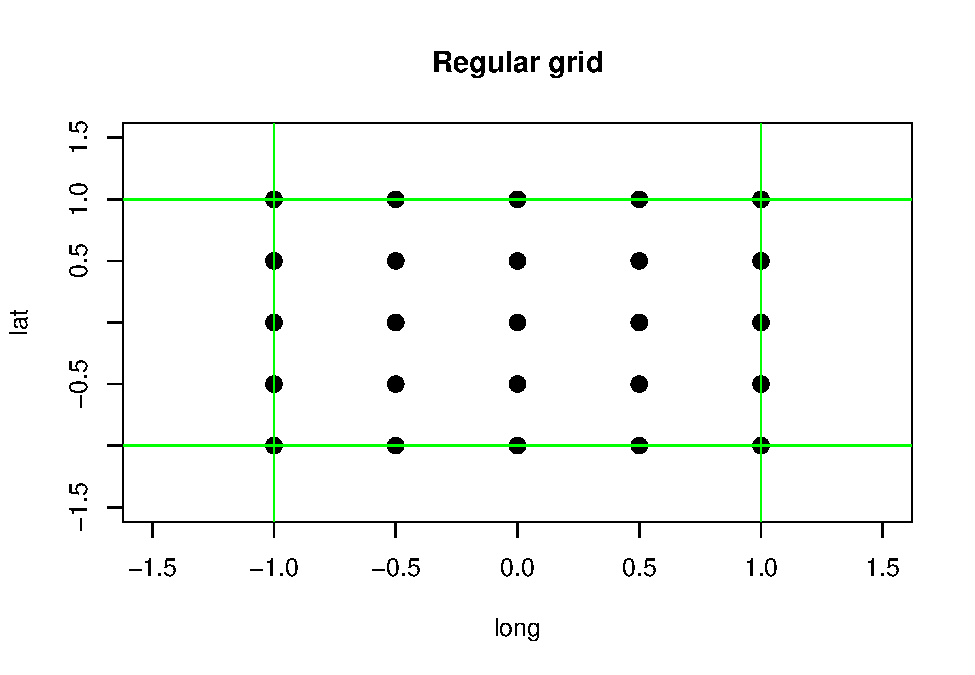
\includegraphics{module1_1_files/figure-latex/unnamed-chunk-46-1.pdf}

It should look something like this (above)!

\paragraph{Finally: some more advanced exploration of
functions}\label{finally-some-more-advanced-exploration-of-functions}

Here is some code to help you get more familiar with some of the less
intuitive aspects of R functions:

\begin{Shaded}
\begin{Highlighting}[]
\NormalTok{#################}
\CommentTok{# More advanced exploration of functions!}

\NormalTok{########}
\NormalTok{## first class functions}

\NormalTok{## assign functions to values}
\NormalTok{sum2 <-}\StringTok{ }\NormalTok{sum}
\KeywordTok{sum2}\NormalTok{(}\DecValTok{1}\NormalTok{, }\DecValTok{2}\NormalTok{, }\DecValTok{3}\NormalTok{, }\DecValTok{10}\NormalTok{)    }\CommentTok{# use the value sum2 as a function!}

\NormalTok{## use functions as arguments in other functions}
\NormalTok{## lets compute the average length of some of the vectors we've created}
\NormalTok{## this should return 3.66}
\KeywordTok{mean}\NormalTok{(}\KeywordTok{c}\NormalTok{(}\KeywordTok{length}\NormalTok{(vector1), }\KeywordTok{length}\NormalTok{(vector2), }\KeywordTok{length}\NormalTok{(vector3)))}
\end{Highlighting}
\end{Shaded}

Let's walk through this last line of code together. We are use 3
different functions: \texttt{c}, \texttt{length}, \texttt{mean}.
\texttt{length} is calculating the length of each vector. We are then
taking the results of length and creating a vector with the \texttt{c}
functions. The result of this is then used as the argument for the
\texttt{mean} function.

Throughout your R journey you will see these properties used many times.
Maybe not so much when first starting. But they are important concepts.
Especially the fact that the R has first-class functions. Functions are
often used as arguments to other functions as a shortcut. It saves the
intermediate step of saving the results to another variable, then
providing that variable as an argument. It also tends to save memory, as
we are no longer storing that variable in memory.

\href{module1_2.html}{--go to next module--}


\end{document}
